\documentclass[11pt]{article} % Adding 'twocolumn' for two-column layout
\usepackage[margin=0.75in]{geometry} % Setting custom margins
\usepackage{amsmath}
\usepackage{graphicx}
\usepackage[numbers]{natbib} % Enabling numeric citations with natbib
\usepackage{float}
\usepackage{url} %for urls on bibtex file

\title{[18F]FDG-PET/CT in Pancreatic Cancer: Challenges and Advances}
\author{Daniel Juarez}
\date{\today}

\begin{document}

\maketitle

\section{Introduction}

Pancreatic cancer is a type of cancer that starts to spread out form the pancreas. The pancreas is situated behind the stomach and its functions include secreting of digestion enzymes and regulating blood sugar. What makes pancreatic cancer really serious is its \textit{poor prognosis} this means that compared to other cancers this one is harder to treat successfully, harder to detect or prevent from growing.

This type of cancer is one of the most challenging in the field of oncology, it has a notably high mortality rate and low survival rates. In the US, pancreatic cancer is currently the 10th most commonly diagnosed cancer, with an estimated 66,440 new cases anticipated in 2024, accounting for 3.3\% of all new cancer cases \cite{SEER2024}. The incidence rate is about 13.5 per 100,000 men and women, with annual increases of about 1\% since the early 2000s. And sadly, it is responsible for 8.5\% of all cancer-related deaths, with an estimated 51,750 deaths expected in 2024 \cite{SEER2024}.

This similar scenario is observed across the world, for example in Mexico it ranks 12th in incidence, and 7th in mortality \cite{GlobocanMexico}. In China incidence ranks 8th. Overall, Pancreatic cancer is the fifth most common cause of cancer-related deaths in South Korea, and the fourth leading cause of cancer-related deaths in the US and Europe. \cite{NCCNGuidelines}
 
 Moreover, pancreatic ductal adenocarcinoma (PDAC), one of the most lethal human cancers that conforms 85\% of pancreatic cancers, is estimated to be the second leading cause of cancer-related deaths by 2030. \cite{Li2022}\cite{Cancers2023}.

 This is a general concern for health professionals and it reflects the limited or "slow" advances in diagnosis and treatment for this malignancy.

%\subsection{Challenges in Early Detection}

Given this statistics, it is crucial for us to quickly identify and treat this type of cancer. This can be quite challenging as it has an aggressive nature and asymptomatic progression. Usually this malignancy doesn't manifest and this leads to diagnoses in more advanced stages and by then surgery is rarely viable \cite{Pubmed30721664}.

There specific reasons why PDAC early detection is challeging has its root in different factors. On the clinical side of things, the initial stages of pancreatic cancer often go unnoticed as symptoms are minimal and non-specific. This early stage end quickly, the rapid progression and agrassive nature of the disease contributes to the complexity, by this time symtoms are noticible but may be to late.   Additionally, the deep location in the anatomy of the pancreas complicates physical examination. 

On the technical part, unlike other malignancies, pancreatic cancer lacks a standardized and reliable screening protocol for the general population, reducing the likelihood of early intervention. Futhermore, existing imaging modalities often fail to detect smaller lesions or early-stage pancreatic cancer \cite{Pubmed30721664}.It is worth pointing out that even surveillance with available techniques is sometimes not recommended if the patient has not developed any symptoms.

Given these diagnostic limitations, there is an increasing demand for imaging solutions can appropriately stage the disease and detect it early in order to improve patient outcomes. Recent literature emphasizes the need for screening programs for asymptomatic, high-risk individuals with non-invasive precursor lesions, rather than those in advanced stages \cite{Cancers2023}.



%\subsection{The Role of Imaging in Pancreatic Cancer Management}

Now, how can we detect this malignancy given all this challenges? Medical imaging is particularly useful in this case, it is able to provide information for treatment planning and assessing resectability. Current guidelines, including those by the National Comprehensive Cancer Network (NCCN) and the European Society for Medical Oncology (ESMO), point out that computed tomography (CT) is the primary imaging modality for assessing pancreatic cancer \cite{NCCNGuidelines}. However, emerging modalities such as endoscopic ultrasound (EUS) and magnetic resonance imaging (MRI) are quickly being more common as supplementary techniques for early-stage evaluation. There is data that compares these modalities in terms of strength, weaknesses and performance that suggests that a hybrid approach like PET/CT will allow for the detection of increased glucose metabolism, offering insights beyond structural abnormalities. \cite{life13102044}

\subsection{FDG PET/CT}

A promising modality for cancer diagnosis and staging is Positron emission tomography/computed tomography (PET/CT). While PET scans are able to capture cellular metabolic changes, CT provides anatomical mapping, this hybrid approach of techniques enables a complete assessment of the disease. Recent studies explore the main advantages and procedures involved using PET/CT with 18-fluorodeoxyglucose ([18F]FDG) a tracer to asses pancreatic cancer. They highlight that the unique advantage of [18F]FDG-PET/CT is in its sensitivity to the metabolic activity of cancer cells, providing valuable insights into both the presence of tumors and their potential aggressiveness \cite{Pu2021}.

Because of the asymptomatic and aggressive nature of PDAC, giving a clear diagnostic is challenging even now with imaging modalities. The advancements in this modalities like [18F]FDG-PET/CT, are very promising improving early detection rates and treatment outcomes. This paper will explore the current applications of [18F]FDG-PET/CT in pancreatic cancer diagnosis and staging, with a focus on overcoming diagnostic limitations and enhancing the accuracy of early detection.

%Section 2: Why PDAC is hard to image (biology-driven challenges).
    
\section{The Nature of Pancreatic Cancer}

%pancreas anatomy

The pancreas is an accesory organ of the digestive system, just like the liver, the gallbladder and salivary glands. The pancreas is located in the upper abdomen retroperitoneally, that is behind the peritoneum, the tissue that lines the abdominal wall and covers most of the abdominal organs \cite{talathi2023}, as shown in figure \ref{fig:pancreas_position}. 


\begin{figure}[h!]
	\centering
	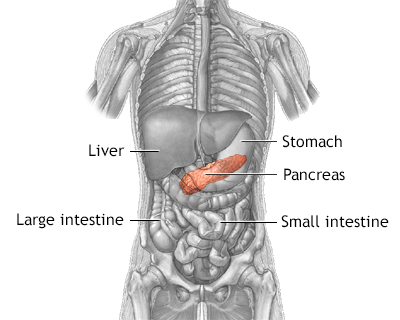
\includegraphics[width=0.5\textwidth]{assets/8883.png}
	\caption{The position of the pancreas in the body and its surrounding organs. Source: \cite{mountsinai_pancreatic_position}.}
	\label{fig:pancreas_position}
\end{figure}

It has 3 main parts, the head lies within the C-shaped curve of the duodenum and the body and tail extend across the midline towards the spleen. \cite{kenhub_pancreas} The division of the pancreas into three main parts (head, body, and tail) helps understand its vascular anatomy too. This is important since radiotracers find their target through this pathways. 

The pancreas receives blood from multiple sources, for example the head gets blood from the superior and inferior pancreaticoduodenal arteries and then drains via the superior mesenteric vein. The suppliers of blood for the body and tail are branches of the splenic artery and drains through the splenic vein. \cite{talathi2023,kenhub_pancreas}

Another relvant part of the pancreas are its ductal system, the main pancreatic duct (Wirsung duct) runs the length of the pancreas and joins with the common bile duct to form the hepatopancreatic ampulla (ampulla of Vater).\cite{kenhub_pancreas} Depicted in figure \ref{fig:pancreas_ducts} as pancreatic duct and Orifice of common bile-duct. 

\begin{figure}[h!]
	\centering
	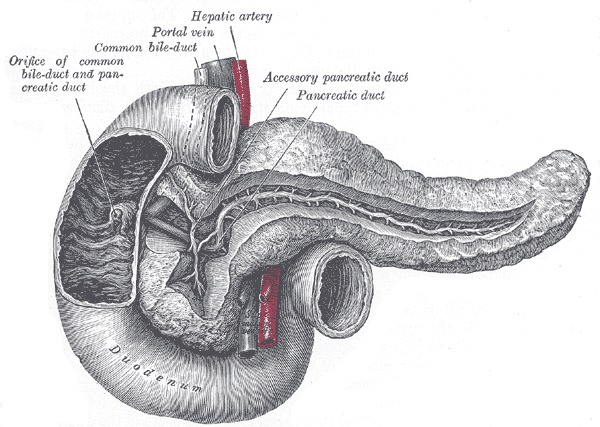
\includegraphics[width=0.5\textwidth]{assets/Gray1100.jpg}
	\caption{The pancreas and its ducts, arteries, and veins. Image by Henry Vandyke Carter, Public Domain, via Wikimedia Commons. Source: \cite{gray_pancreas_ducts}.}
	\label{fig:pancreas_ducts}
\end{figure}

%where PDAC originates

Pancreatic ductal adenocarcinoma (PDAC) is a highly aggressive malignancy and is characterized by rapid progression. It has distinct biological and structural features, the relevant ones for imaging it are two, altered glucose metabolism (metabolic reprogramming) and a dense fibrotic tumor microenvironment. These characteristics create significant challenges for traditional imaging modalities, thus medical physicists and physicians require advanced techniques like PET/CT for accurate diagnosis.

The disease can manifest anywhere in the pancreas but most PDACs (60-70\%) arise from the head. While 20-25\% of PDACs originate in the body or tail of the pancreas. Tumors in the pancreatic head tend to be diagnosed earlier due to their proximity to the common bile duct \cite{stark2015}.

PDAC arises from cells of the pancreatic duct or ductules   \cite{stark2015}. The tumor is often surrounded by a prominent desmoplastic stroma,a dense connective tissue growth, which contributes to its aggressive behavior \cite{haeberle2019}. Because of this, vascular invasion is common, occurring in about 65\% of cases, and is associated with poorer prognosis \cite{hong2012}. Also, as illustrated by figures \ref{fig:pancreas_position} \& \ref{fig:pancreas_ducts} the pancreas has very imporant surrounding structures meaning that PDAC can directly extend into nearby organs like the spleen, adrenals, stomach, and transverse colon. \cite{radiopaedia_pda}

%\subsection{Metabolic Reprogramming in PDAC}

PDAC tumors have metabolic alterations, explained by the Warburg effect.\cite{Hammond2024} The Warbug effect occurs when cells change to a sugar-based energy pathway, over oxygen-based ATP production, even in oxygen-rich conditions. ATP, the molecule cells use for energy, is normally generated through oxygen-driven processes, but glycolysis allows tumor cells to grow rapidly. This shift is driven by genetic mutations associated with cancer, such as KRAS, which increase the production of glucose transport proteins (GLUT1) and processing enzymes (hexokinase-2), this allows for cell proliferation and growth. \cite{Pubmed30721664, Pu2021}.

%what does the images must reveal?

PET/CT imaging for pancreatic lesions must reveal several key features to aid in diagnosis. First, from PET images elevated FDG uptake compared to benign lesions is expected, as cancer cells typically exhibit increased glucose metabolism. This scanner can detect the accumulated hyperglycolytic tumor cells, via the radiotracer [18F]FDG, a glucose analog, meaning it can detect PDAC lesions, with sensitivity rates of 89–91\% and specificity rates of 70–72\% in clinical applications \cite{Pu2021}.

The scan needs to provide information on the size and location of the lesion, as well as any presence of cystic necrosis, since is more common in PDAC (59.6\% of cases). Some other important infomation that can be extracted from a PET/CT scan is the spread of the disease, via vascular invasion or metastases on liver or peritoneal \cite{parikh2020fdg}.  

%how does CT help?
Usually, on a conventional PET/CT protocol, a CT scan is perfomed without any alteration. From this scan, data on the attenuation coefficients are obtained and it alows to correct PET images later. It also provides anatomical localisation, so the high FDG part can be identified \cite{benamor2007petct}. Recent studies explore the newest techonology that is used to diagnose PDAC, that include MRI with Diffusion weight imaging (DWI) and Dynamic Contrast Enhance (DCE), elastography and nanoparticles. \cite{Cancers2023}

% differences with pancreatitis

A main challenge for diagnostics from these images is differentiating PDAC from pancreatitis. The tumor size in mass-forming chronic pancreatitis (MFCP) tends to be larger (mean size $4.00±0.47$ cm) compared to PDAC (mean size $3.42±0.75$ cm) \cite{arnone2020}. But those values are pretty close to eachother pointing that diagnosing out of only tumor size is nearly impossible. 

Thankfully, we got some other data to help distinguish between the two. An example is that, PET/CT can better detect vascular invasion, which is more common in PDAC (53.2\%) than in MFCP (23.8\%). And other factors like cystic necrosis and atrophy can also play a role, since these factors and More frequently observed in PDAC than in MFCP \cite{arnone2020}. 

A key factor is that PDAC typically shows higher FDG uptake (higher SUVmax) compared to MFCP due to increased glucose metabolism in cancer cells \cite{arnone2020,Pu2021}. However, even with this metrics diagnostics is quite challenging, as we will explore in a later section on this paper.


%\subsection{Tumor Microenvironment and Imaging Challenges}

Thick fibrous tissue (desmoplastic stroma) surrounds cells in organs, is made up of fibroblast cells and extracellular proteins like collagen. In normal tissues, it provides structure and helps supply nutrients to healthy cells. However, in cancer the stroma becomes abnormally dense and fibrotic. This is called desmoplasia and helps the tumor grow and evade immune attacks, for imaging purposes, this thick tissue also makes it harder for CT and MRI to clearly identify the tumor's boundaries \cite{NCCNGuidelines}.


Additionally, hypoxic regions within the tumor alter glucose metabolism, causing variability in [18F]FDG uptake. This will be discussed in depth later in this document. Making imaging more complicated, inflammatory conditions, such as pancreatitis can produce lesions with overlapping metabolic signatures on PET/CT. As noted by Pu, Y. \cite{Pu2021}, ``both autoimmune pancreatitis and pancreatic cancer appear as metabolic abnormalities and increased FDG accumulation''.


%\subsection{Advanced Imaging Needs}

The challenges presented above highlight the need of development on advanced imaging modalities to ensure accurate diagnosis and staging of these types of cancer. PET/CT combines the sensitivity of metabolic imaging with the spatial resolution of CT, and has emerged as a strong candidate for precise tumor localization and characterization.

Recent studies agree on this and are doing research on the topic. Stating that "The combination of PET and CT can determine the metabolic capacity and anatomical position of pancreatic tumor cells in the body and can accurately diagnose the patient's condition and tumor location" \cite{Pu2021}. Other research shows interest in different modalities, such as PET/MR and the use of other radiotracers for targeting hypoxic or stromal regions. But they all agree that development is needed. This development hold promise for enhancement in diagnostic specificity and sensitivity, although they require validation in clinical settings \cite{Cancers2023}. 

%What could MR offer?

For comparative analysis on PET/MR and PET/CT in therapeutic applications, see also \cite{myownotherpaper}. Where an exploration on what MR offers is included. The main advantages that MRI can add are reduced dose when compared with PET/CT and as an standalone modalitie, the DWI \& DCE allows for additional functional information on the ducts and viens of the accesory digestive system organs to be obtained.


\subsection{The Importance of Early Detection}

Patient outcomes depend entirely on the capacity to early detect pancreatic ductal adenocarcinoma (PDAC). Despite advancements in therapeutic strategies, over 80\% of PDAC patients have locally advanced or metastatic disease at the time of diagnosis, at this stage the curative options are limited. Early-stage detection allows for timely surgical resection, the only potentially curative treatment that improves survival rates \cite{Cancers2023}. 

Because fo the asymptomatic progression and aggressive nature of PDAC its early detection is extraordinarily difficult. Current technology and traditional imaging techniques, like CT and MRI, offer insights when assessing this disease but are limited by heir ability to identify small lesions or distinguish benign from malignant tumors early on. This cases are well illustrated in resource-limited settings, if PET/CT is scarce this challenge becomes even more daunting. For instance, in Mexico PET scanners are centralized in major cities and early detection relies heavily on less sensitive modalities like CT or X-ray, which are often insufficient for timely diagnosis.

The reality of this worldwide problem is showcased in many real-world cases, a personal example is that of my grandmother, whose diagnosis of PDAC came only after her passing, despite months of observation and testing.

Better imaging modalities, such as [18F]FDG-PET/CT, can address some of these issues. The combination of functional and anatomical imaging improves sensitivity and specificity for early lesions, thus enables metabolic changes to be detected before morphological alterations appear \cite{Pu2021}. However, access to these technologies remains uneven globally. As of 2021, Mexico had only 26 PET scanners for its entire population, around 126 Million people \cite{inegi_population}, concentrated in a few hospitals in major cities \cite{statista1}. There is a need for international collaboration to expand access to advanced imaging technologies, both through equipment and expertise.


Another proposed solution to these problems is the addition of surveillance for high-risk groups, with population-specific screening programs targeted to individuals with familial predisposition, cystic lesions, or diabetes mellitus in order to identify precursor lesions or early-stage PDAC \cite{Cancers2023}.

Furthermore, these programs are limited in settings where resources are lacking. Following my personal story, that of my grandmother, who was a high-risk patient with diabetes and a delayed diagnosis, exemplifies the need for accessible and standardized surveillance protocols. The value of those programs not only relies on saving lives but on valuable insights into familial risk factors, which is an area of interest for researchers and patients alike.

When PDAC is diagnosed at a localized stage, surgical resection is more likely to be feasible. Advanced imaging techniques like [18F]FDG-PET/CT offer the potential to identify tumors earlier. Expanding access to these technologies and implementing population-specific screening programs puts the world in the right direction to address this global health challenge and improve outcomes for future patients.

%Section 3: How PET/CT overcomes those challenges (physics and technical focus).
\section{Overview of Imaging and [18F]FDG Tracer}

\subsection{Technical Principles of PET/CT}

Positron Emission Tomography (PET) is a functional imaging modality that uses positron-emitting radionuclides to map metabolic activity in tissues. As standalone imaging modality it lacks of anatomic structure localization, for that it is integrated with Computed Tomography (CT). CT contribution is huge, it provides attenuation correction, electron density, and anatomical localization. This way, PET/CT provides both functional and structural data in a single imaging session and with it a valuable approach in planing and diagnosing. With the use of PET annihilation gamma rays and CT high resolution it is possible to find accurately the localization of metabolic abnormalities \cite{TG174}. By taking the best of both modalities it is ensured that all metabolic information is properly contextualized on the anatomy reducing errors on registration state compared to standalone systems \cite{TG126}.

%CT
% Resolution required?

%Physics of PET/CT
%how is this acomplished
% scanner config
%technical details
%why both

The now well established Time-of-flight (TOF) technology allows to get precise timing of gamma-ray detection to improve spatial resolution and reduce noise. As it solves the problem of measure the exact site of anihilation it enchances ignal-to-noise ratio (SNR), particularly for larger patients. \cite{Seifert2022} PET technology has advanced a lot in recent years with detection enhancement, such as the adoption of Silicon Photomultiplier Arrays (SiPM) replacing older photomultiplier tubes (PMTs) augment resolution and sensitivity \cite{SunderlandSeminar}. And with it the regulations and quality assessments ensure that metrics like Standardized Uptake Value (SUV) are reliable.\cite{TG174}.

Additionally, there is another important factor related to PET scanners, as PET imaging requires administration of radiopharmaceuticals. This administration must be performed with accuracy as any error in this step, can lead to uneven tracer distribution. The next section will explore more about the particular radiotracer [18F]FDG. Sunderland et al. demonstrated that injection infiltration occurs in less than 0.4\% of cases. Moreover, computational modeling suggests that even when infiltration occurs, its impact on dosimetry and image quality is negligible  \cite{Sunderland2023}. 


\subsection{Mechanism of [18F]FDG Uptake}


Fluorine-18 Fluorodeoxyglucose or [18F]FDG is a glucose analog labeled with the positron-emitting isotope fluorine-18. After intravenous injection, FDG is transported into cells by glucose transporters like GLUT1 and  the enzyme hexokinase adds a phosphate group (phosphorylase) to it. Since this is now a different molecule from glucose cells cannot longer proceed in the glycolysis process, and the molecule gets trapped in cells with high glucose metabolism, such as tumor cells \cite{TG174, Zheng2018}.

This characteristic of the cancer cell is what allows for PET to visualize regions of hyperglycolysis. For example, as shown in Figure \ref{fig:PuFig1}, PET images A) show regions of increased metabolic activity in the pancreatic head, in B) CT images provide anatomical context. The fused PET/CT image C) integrates these modalities, and allows for precise localization of pancreatic tumors.
Then oncogenic mutations like KRAS drive this process by upregulating GLUT1 and hexokinase-2, further amplifying glucose uptake \cite{Deng2021}. But this is not the only reason FDG accumlation can increase, this behaivior is also present in inflammation and benign conditions, such as autoimmune pancreatitis \cite{Zheng2018}. Different radiotracers may shine some light into the problems faced right now and and with them new advancements in tracer specificity and imaging protocols emerge.

\begin{figure}[ht]
    \centering
    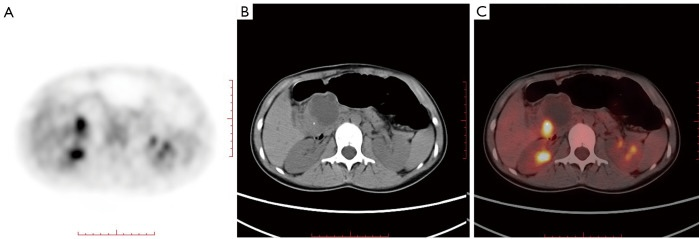
\includegraphics[width=0.8\textwidth]{assets/tcr-10-07-3560-f1.jpg}
    \caption{18F-FDG PET/CT imaging integrating metabolic and anatomical data: (A) PET image, (B) non-enhanced CT image, (C) fused PET and CT images, demonstrating pancreatic head cancer detection \cite{Pu2021}.}
    \label{fig:PuFig1}
\end{figure}

\section{Applications in Staging and Diagnosis}

With the complementary strengths of PET and CT scanners assessing tumor margins and guiding surgical interventions is possible. In the case for staging and diagnosing PDAC, PET/CT achieves sensitivity rates of 89–91\% and specificity rates of 70–72\% in detecting PDAC lesions \cite{TG174}.

Key applications include:
\begin{itemize}
    \item \textbf{Tumor Localization and Metastases Detection}: PET/CT excels in identifying primary tumors and distant metastases by FDG concentrated regions lighting up. Zhang et al. demonstrated its utility in detecting rare metastatic sites, such as cutaneous and muscle involvement\cite{Zhang2023}.
    \item \textbf{Lymph Node Evaluation}: In cancer, lymph nodes often act as early sites for metastasis. PET/CT is a great tool to assess lymph node involvement. When FDG concentrates it shows increased glucose metabolism due to cancer activity. This is unique information from PET since lymph nodes may appear normal in size on CT but are metabolically active. Accurate identification of these cancerous nodes improves staging precision, which is critical for planning surgeries, such as lymphadenectomy (removal of affected nodes), and for deciding if curative treatments are feasible \cite{TG174}.
    \item \textbf{Differentiating Lesions}: Since FDG uptake is non-specific, combining metabolic imaging with clinical markers (e.g., IgG4 levels) can help distinguish autoimmune pancreatitis from PDAC \cite{Zheng2018}.
\end{itemize}

Another one of the emerging technologies is the Total Body PET/CT systems. This systems seek to enable whole-body imaging in a single scan, hopefully with enhanced resolution and reduced scanning time \cite{SunderlandSeminar}. This is a valuable innovation for detecting micrometastases and monitoring therapeutic responses. %how is different from normal?

%\section{Applications of [18F]FDG-PET/CT}

PET/CT can be of great help during the different parts of treatment, from diagnosis, staging, to management of pancreatic cancer. In order to exemplify its applications three clinical cases are introduced:

\begin{itemize}
    \item \textbf{Case 1 - Zheng et al.:} 
    A 67-year-old male  with suspected pancreatic cancer presented, in 2018, a metabolic active lesion was identified using a PET/CT scanner. This lesion is located in the head of pancreas and had hinted overlap of metabolic signatures typical of both malignancy and autoimmune pancreatitis\cite{Zheng2018}.
    \item \textbf{Case 2 - Zhang et al.:} 
    In 2023 case, a 64-year-old male with confirmed pancreatic adenocarcinoma and treated with radical resection 6 years earlier presented rare metastatic sites and was reevaluated\cite{Zhang2023}.
    \item \textbf{Case 3 - Deng et al.:} 
    Study in 2021 that compared FDG with 68Ga-FAPI, Gallium-68-labeled Fibroblast Activation Protein Inhibitor, in a 58-year-old female with pancreatic cancer and liver metastases. DG-PET/CT identified hypermetabolic liver lesions, but 68Ga-FAPI demonstrated superior sensitivity in delineating hypodense metastases\cite{Deng2021}.
\end{itemize}

These cases together exemplify applications in the diagnosis and staging of pancreatic cancer of this imaging modality.

\subsection{Tumor Localization and Metabolic Assessment}

\textbf{Metabolic Imaging in Practice:} As stated before the value of FDG-PET resides on the its ability to visualize regions of increased glucose metabolism, even in lesions not that well defined morphologically. A case application is the results of Deng et al. where FDG-PET/CT effectively detects hypermetabolic pancreatic tumors. But, new tracers like 68Ga-FAPI outperform FDG in identifying micrometastases, particularly in hypodense liver lesions \cite{Deng2021}. %differences on the isotope

Figure~\ref{fig:DengMerged} illustrates the comparative uptake of 68Ga-FAPI and 18F-FDG in pancreatic cancer with liver metastases, the maximum density projection (MIP) image (A) shows increased FDG uptake in a pancreatic mass and mild uptake in the 10th rib, suggesting bone metastasis. Axial PET/CT images (B) highlight moderate uptake in the pancreatic head, while (C) reveals minimal bone destruction with mild metabolic activity in the 10th rib. Additionally, small hypodense nodules in the liver (D) were identified without significant FDG uptake, raising suspicion for liver metastases.

\textbf{Quantitative Metrics in Action:} The metric of choice is the Standardized Uptake Value (SUV), it measures FDG uptake in a lesion relative to a reference. The lower the SUV the better as it correlates to malignancy. By knowing this parameter it is posiible to identify micrometastatic lesions, particularly in the liver. Deng et al. shows that 68Ga-FAPI has superior sensitivity highlighting it as a promising area for future research on radiotracers.\cite{Deng2021}


% walk thru
\begin{figure}[ht]
    \centering
    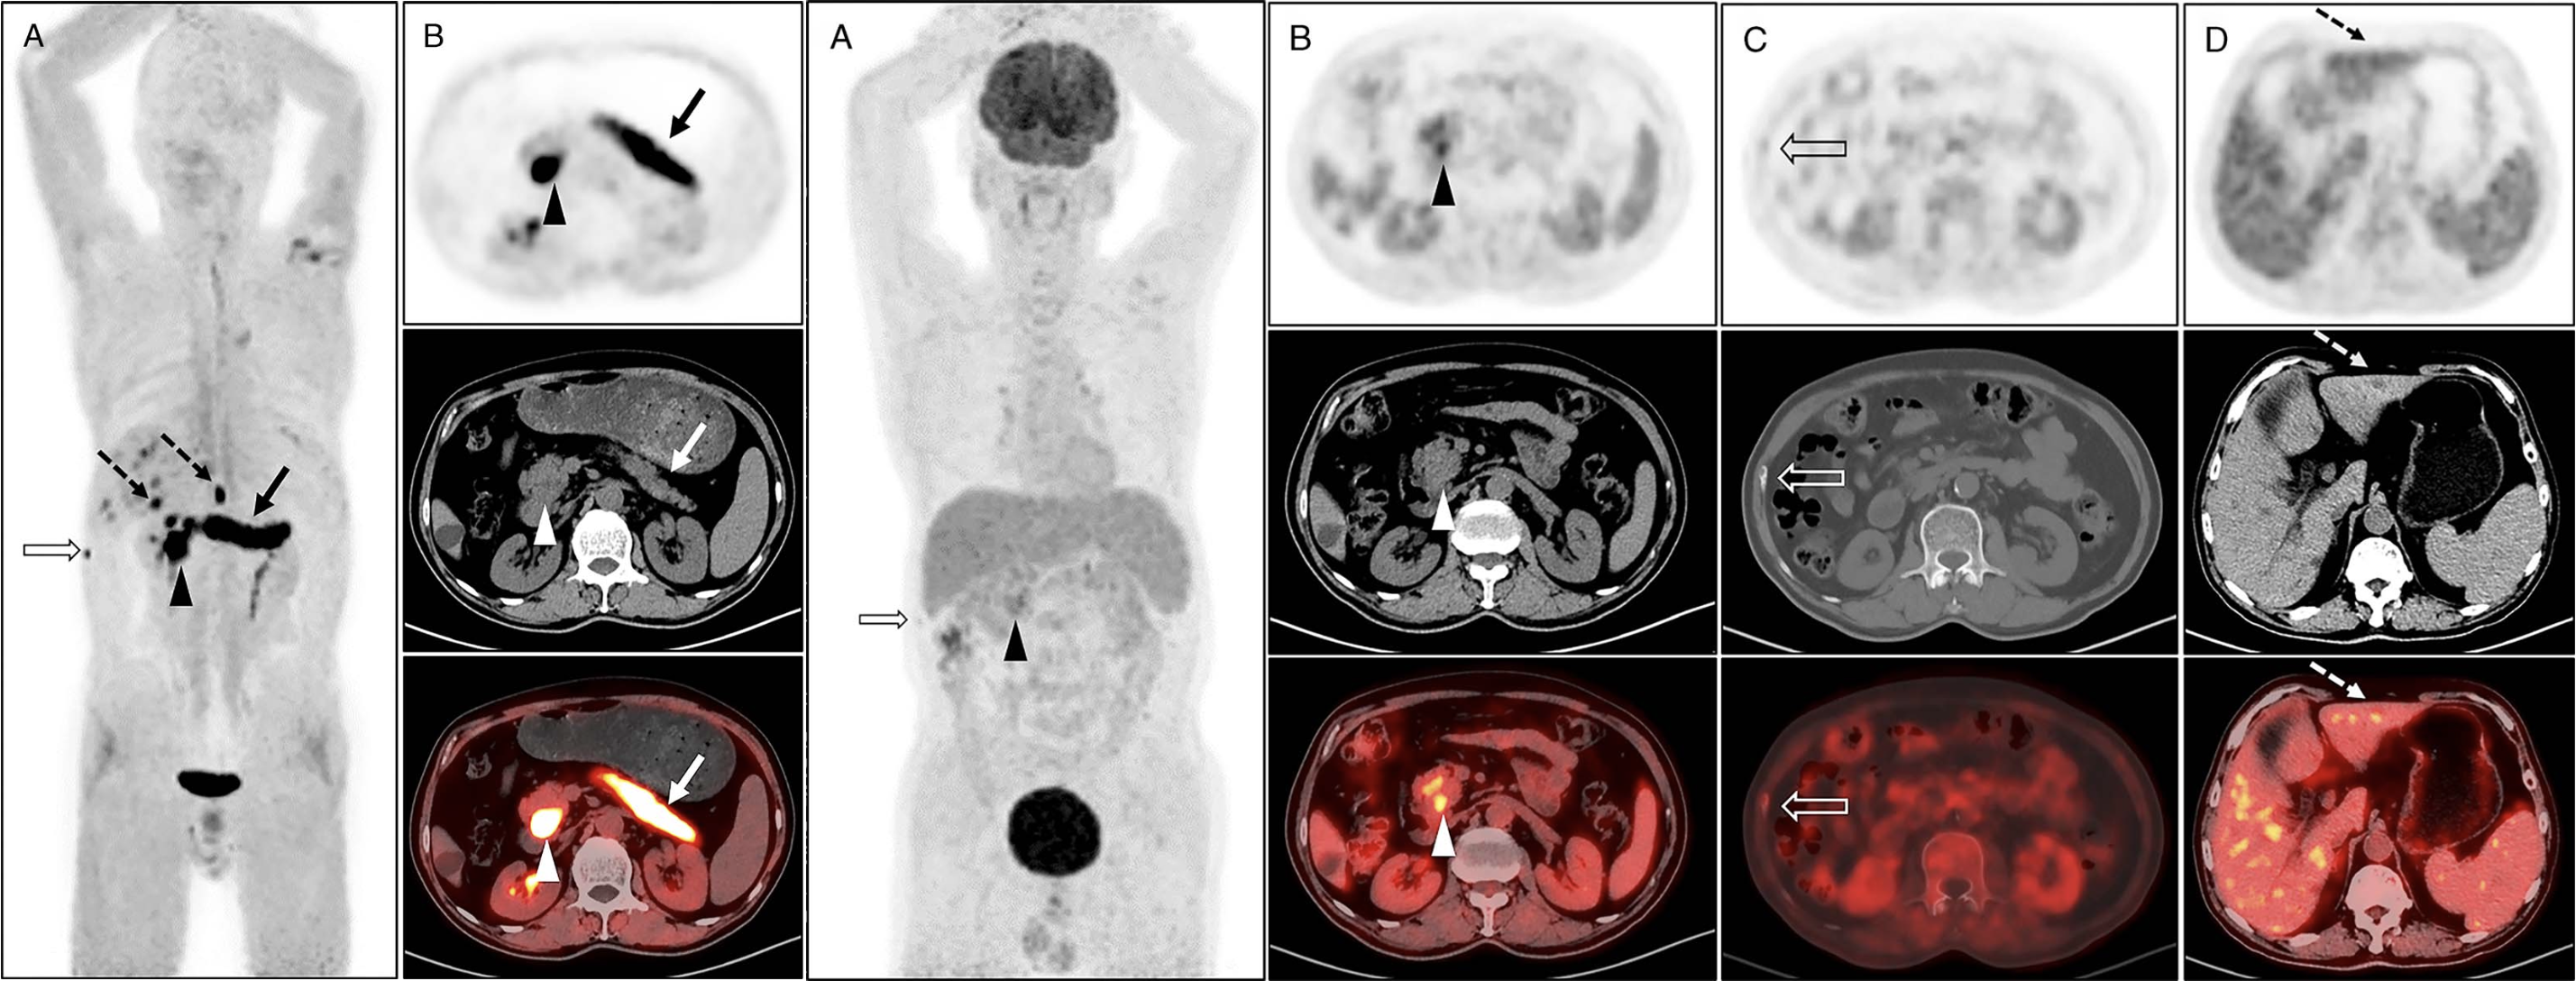
\includegraphics[width=0.9\textwidth]{assets/DengMerged.png}
    \caption{Comparison of FDG-PET/CT metabolic activity. (Right) 18F-FDG PET/CT showing pancreatic mass and liver hypodense lesions with minimal uptake, highlighting its sensitivity in tumor and liver staging \cite{Deng2021}. (Left) Enhanced metabolic activity in pancreatic lesions with high resolution, 68Ga-FAPI tracer’s specificity in hypometabolic areas near liver\cite{Deng2021}.}
    \label{fig:DengMerged}
\end{figure}

%---

\subsection{Lymph Node Evaluation and Metastasis Detection}

\textbf{Unique Metastases:} 
In case 2, PET/CT demostrated its capacity to distiguish between muscle and cutaneous metastases from PDAC—locations rarely detected by conventional imaging. Without PET/CT this would be possible to asses correctly

Figure~\ref{fig:Zhang1}, depicts a MIP image with two regions of elevated glucose metabolism (Upper abdomen and left lateral abdominal wall). An axial image of the anatomy shows near the surgery site that shows elevated metabolic activity, possibly indicating residual or recurrent cancer, or post-surgical inflammatory changes. Then focused on the lateral it shows an hypodense structure seen in the muscle. This is the rare case of a metastatic deposit in the muscle. They highlight that Muscle metastases from pancreatic cancer are exceptionally rare, while cutaneous metastases occur in only 0.5–7.6\% of cases, often at the umbilicus\cite{Zhang2023}.


\textbf{Sensitivity and Specificity:} Zhang et al. found that FDG uptake reliably identifies malignancies, it may also highlight non-malignant inflammatory processes, necessitating careful interpretation and, when possible, the inclusion of additional clinical markers or advanced tracers.

\begin{figure}[H]
    \centering
    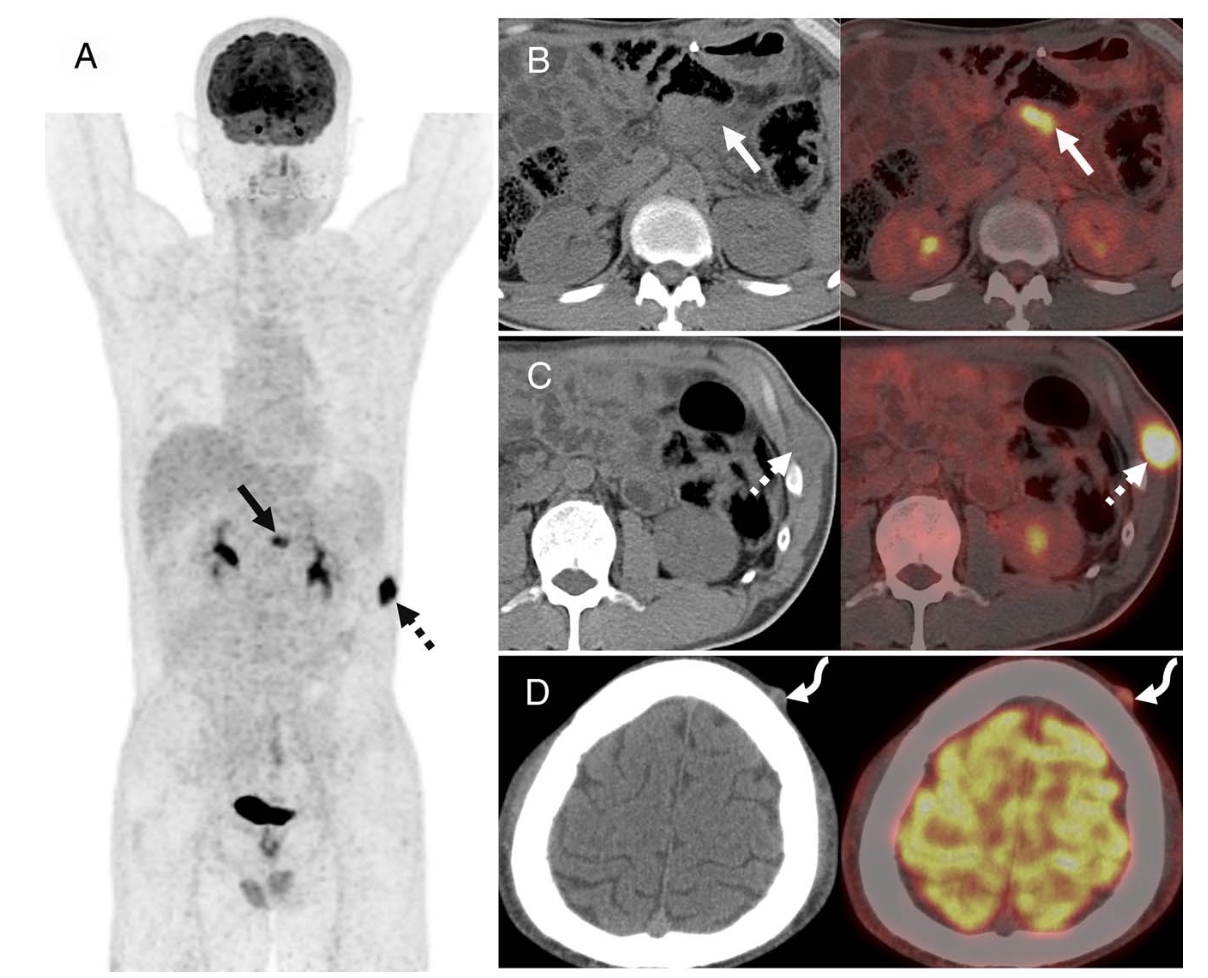
\includegraphics[width=0.8\textwidth]{assets/Zhang1.png}
    \caption{Rare cutaneous and muscle metastases detected using FDG-PET/CT, illustrating its capability for identifying uncommon metastatic sites \cite{Zhang2023}.}
    \label{fig:Zhang1}
\end{figure}

%---

\subsection{Treatment Planning and Monitoring}

\textbf{Guiding Therapy with PET/CT:} In order to perform a surgical resection and radiation therapy the boundaries of the tumor must be carfully delinated. Zheng et al. were able to differentiate autoimmune pancreatitis from PDAC from this images, avoiding unnecessary or ineffective treatments \cite{Zheng2018}.

%explain figures
Figure~\ref{fig:Zheng1} showcases how PET/CT identifies metabolic distinctions that inform treatment in challenging cases where inflammatory and malignant lesions overlap. Additionally, post-treatment PET/CT imaging provides insights into metabolic response, that enables clinicians to adjust therapeutic regimens based on observed changes in FDG uptake.

\textbf{Enhancing Planning with Alternative Tracers:} As noted in Deng et al., the integration of new tracers like 68Ga-FAPI offers improved sensitivity in hypoxic tumor regions. \cite{Deng2021}.

\begin{figure}[H]
    \centering
    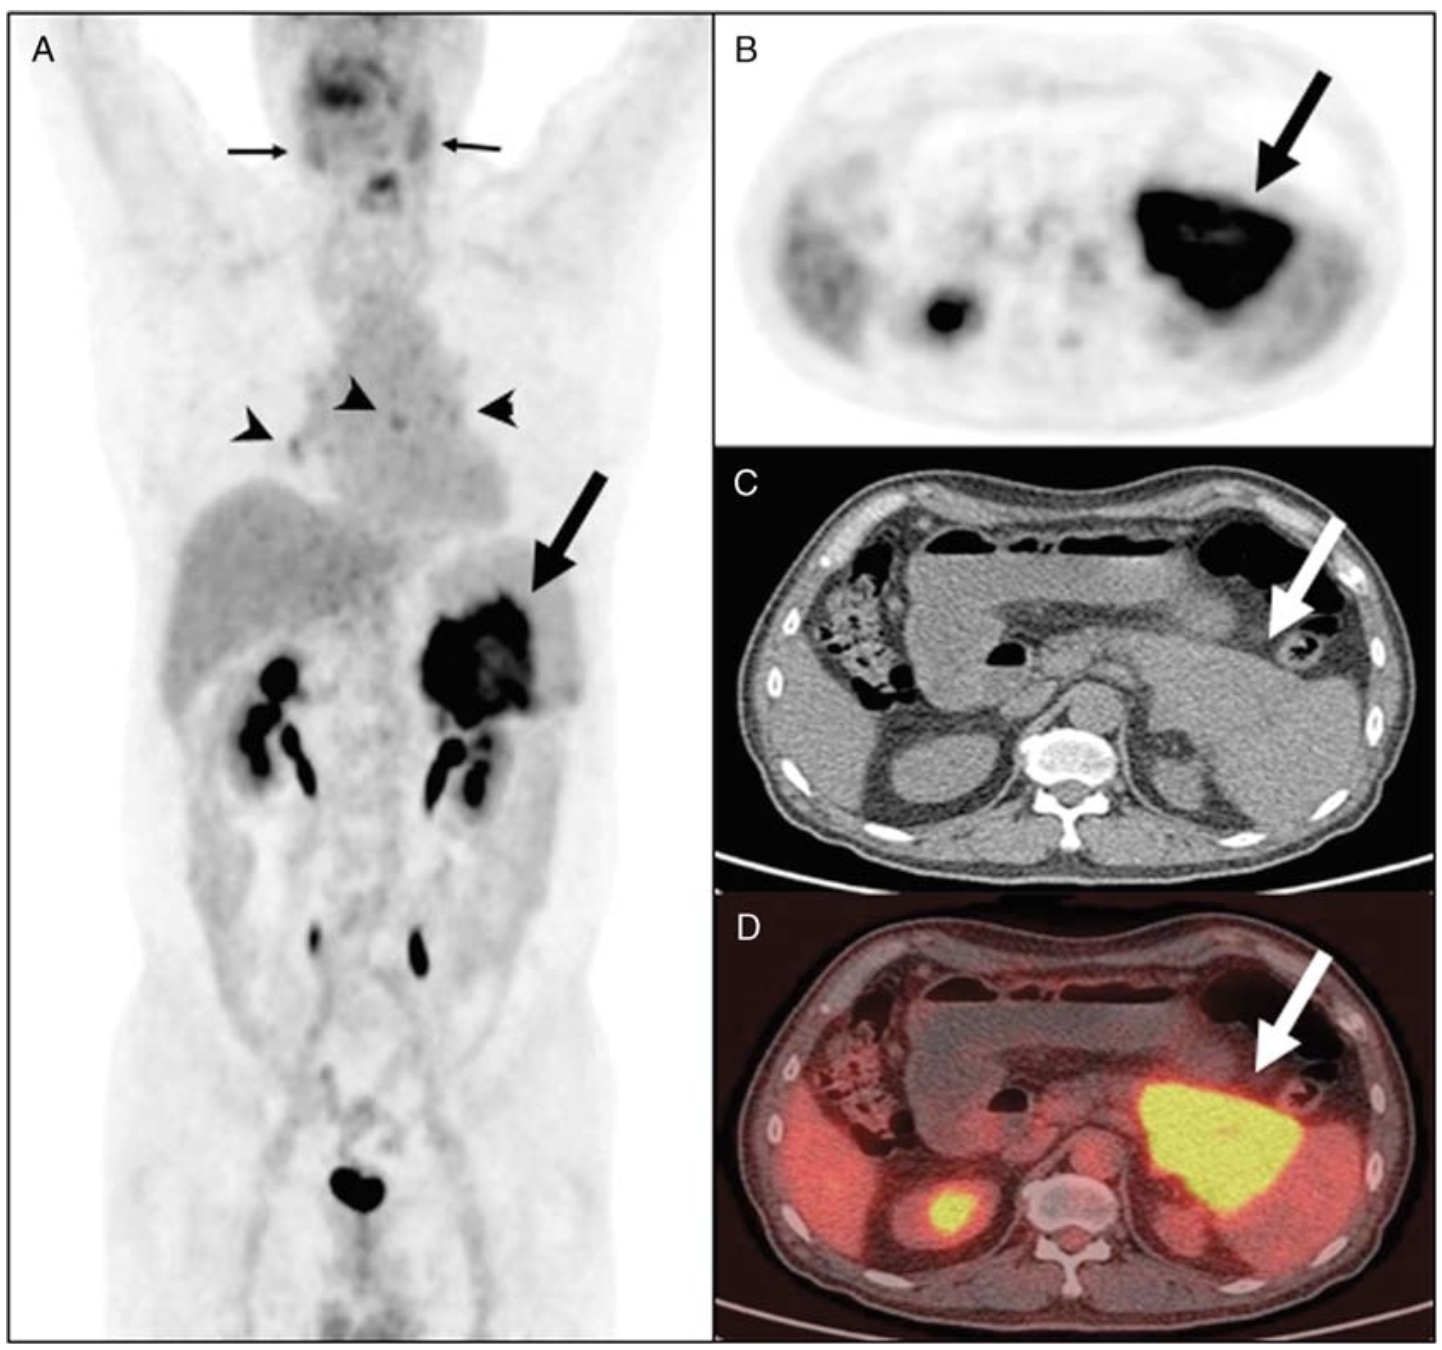
\includegraphics[width=0.6\textwidth]{assets/Zheng1.png}
    \caption{FDG-PET/CT imaging showing focal autoimmune pancreatitis mimicking pancreatic cancer. Note: the overlapping metabolic activity that challenges differentiation \cite{Zheng2018}.}
    \label{fig:Zheng1}
\end{figure}

%---

Section 4 demonstrated the utility that PET/CT provides to diagnosis, staging, and management of pancreatic cancer. These clinical cases are an example of the current technology and limitations that we have in terms of resolution and specificity, and accessibility. Addressing these limitations will lean this technology forward for better and precise treatment, innovations in radiotracer development and hybrid imaging modalities can certainly be the way forward.

\section{Limitations and Future Directions}

\subsection{Current Limitations}

FDG-PET/CT is widely used, but it has limitations. The major one is resolution, this makes detecting micrometastases realky difficult. Another limitation is in the tracer it self, FDG lack the specificity in distinguishing inflammatory from malignant lesions and can lead to diagnostic uncertainty. Furthermore, accessibility remains an issue, as the high costs associated with FDG-PET/CT and its limited availability in certain regions hinder its adoption in resource-limited settings.

\subsection{Future Advancements}

On the side of chemistry and nuclear physics, the development of radiotracers, such as 68Ga-FAPI and [18F]FMISO, offers solutions to FDG’s specificity challenges. These tracers target unique tumor characteristics, such as hypoxia and fibroblast activity \cite{Deng2021}. Then on the resolution problem, technologies like PET/MR provide enhanced soft-tissue contrast and reduced radiation exposure, making them promising alternatives for pancreatic cancer imaging. Additionally, Total Body PET/CT systems promise comprehensive whole-body imaging in a single scan, improving detection of micrometastases and overall efficiency.

%---

\section{Conclusion}

FDG-PET/CT has is a great addition to the diagnostic approach for pancreatic cancer by combining anatomical and metabolic imaging. It has the ability to localize tumors, stage disease, and guide therapy making it a solid choice for oncology assessment. However, addressing its limitations through advanced tracers and hybrid modalities is a priority. The ongoing evolution of PET/CT technology, coupled with global efforts to expand accessibility, will undoubtedly enhance its impact on pancreatic cancer outcomes.

\bibliographystyle{unsrt} % Numbered references in order of appearance
\bibliography{references}

\end{document}